\documentclass[12pt, titlepage]{article}
\usepackage[shortlabels]{enumitem}
\usepackage{booktabs}
\usepackage[normalem]{ulem}
\usepackage{tabularx}
\usepackage{graphicx}
\usepackage{placeins}
\usepackage{geometry}
\usepackage{array}
\usepackage{xcolor}
\usepackage{longtable}
\definecolor{darkgreen}{rgb}{0.0, 0.5, 0.0}

\usepackage{cite}
\usepackage{url}
\usepackage{hyperref}
\hypersetup{
    colorlinks,
    citecolor=blue,
    filecolor=black,
    linkcolor=black,
    urlcolor=blue
}
\usepackage[round]{natbib}

\title{SE 3XA3: Software Requirements Specification\\Supreme Chess}

\author{Team 2, The Triple Grobs
        \\ Jonathan Cels (celsj)
        \\ Pesara Amarasekera (amarasep)
        \\ Rupinder Nagra (nagrar5)
}

\begin{document}

\maketitle

\pagenumbering{roman}
\tableofcontents
\listoftables
\listoffigures

\begin{table}[h]
    \caption{\bf Revision History}
    \begin{tabularx}{\textwidth}{p{3cm}p{2cm}X}
        \toprule {\bf Date} & {\bf Version} & {\bf Notes}\\
        \midrule
        2021-02-11 & 1.0 & Revision 0 of the SRS.\\
        \hline
        \textcolor{red}{2021-04-11} & \textcolor{red}{2.0} & \textcolor{red}{Addressed TA's remarks by changing the document to better match the template given. This included the addition of many sections.}\\
        \hline
        \textcolor{red}{2021-04-11} & \textcolor{red}{2.1} & \textcolor{red}{Made changes to use cases and requirements to match the system, as requirements were altered during the course of the development process.}\\
        \bottomrule
    \end{tabularx}
\end{table}

\newpage

\pagenumbering{arabic}

\section*{Important Information}
    Text that has been struck through, \sout{like this}, was in the previous revision of the document and has been removed. \\
    
    Text that is colored red, \textcolor{red}{like this}, is new to revision 1, and reflects the most recent information. \\
    
    Text that is colored green, \textcolor{darkgreen}{like this}, is a comment to the TA's/professor and should not be included as a part of the content in this document. \\

    \textcolor{darkgreen}{The template was not correctly used for revision 0 of this document. Revision 1 has updated the template to better match the given template. Section and subsection headers that are new to revision 1 are not in red, only the new content of the sections.}\\
    
     \textcolor{darkgreen}{Many functional requirements and use cases were altered or removed. Deleted requirements are struck through rather than removed, so they maintain a requirement name and number even though they are not technically requirements. For example, requirement FR5 no longer exists but there is no new FR5 in order to reduce confusion in traceability.}
    
\section{Project Drivers}

    \subsection{The Purpose of the Project}
        The purpose of this document is to specify the system requirements and how the system interacts with the end user.

    \subsection{The Stakeholders}
        Intended stakeholders for this document include the development team, \textcolor{red}{any end-users}, the professor of the course, and the TAs of the course.
    
        \subsubsection{The Client}
            \textcolor{red}{The clients for this project are the professor and TA's of the course. This is because they have tasked the development team with the creation of the software, and their input is used as direction throughout the development life-cycle.}
            
        \subsubsection{The Customers}
            \textcolor{red}{The customers for this project are any users who wish to play computer chess and chat online.}
            
        \subsubsection{Other Stakeholders}
            \textcolor{red}{Other stakeholders for this project include the development team, who are invested in the success and development of the project.}
        
    \subsection{Mandated Constraints}
        \begin{enumerate}[a)]
        	\item Time constraint: The final product must be fully implemented by the end of the semester.
        	\item Resource constraint: The developers will have limited access to additional resources such as more developers, money, and software management tools.
        \end{enumerate}
        
    \subsection{Naming Conventions and Terminology}
        \begin{enumerate}[a)]
        	\item The Software Requirements Specification (SRS) is a detailed document which describes a software system to be developed.
        	
        	\item The Web Content Accessibility Guidelines (WCAG) \cite{WCAG} are guidelines on making web content more accessible to people with disabilities.
        	
        	\item \sout{Artificial Intelligence (AI) in this document refers to a computer-controlled player.}
        \end{enumerate}
        
    \subsection{Relevant Facts and Assumptions}
        \begin{enumerate}[a)]
            \item It is assumed that the user has access to the required hardware and internet connection required to access and play the game without the hindrance of lag or other issues.
            
            \item It is assumed that the user has access to I/O devices, such as a keyboard/mouse/monitor for a computer, or a touchscreen for a mobile device.
            
        	\item Based on the browser used for the web application, the  \textbf{HTML} and  \textbf{CSS} might be affected. This project will use the assumption that a user will be using the latest version of Google Chrome.
        	
        	\item It is assumed that the user has proficiency in the English language.
        \end{enumerate}
    

\section{Functional Requirements}

    \subsection{The Scope of the Work and the Product}
        The software product will provide the user with an implementation of a chess game. The product aims to provide an interactive and entertaining game-play experience utilizing web programming. The user will be able to play with other users online.
        
        \subsubsection{The Context of the Work}
            \begin{figure}[h]
                \centering
                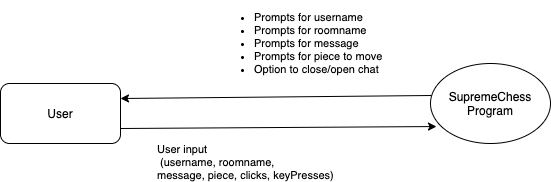
\includegraphics[width=30em]{ContextDiagram.png}
                \caption{Context Diagram}
                \label{fig:usecase}
            \end{figure}
        \subsubsection{Work Partitioning}
\FloatBarrier
    \begin{table}[!h]
    \centering
     \setlength{\leftmargini}{0.4cm}
    \begin{tabular}{| m{2cm} | m{3.3cm} |m{10cm} |}
    \hline
    \textbf{Event Name} & \textbf{Input/Output} & \textbf{Summary}
 \\ 
    \hline
    User enters username & Username(IN) & The user inputs a username to identify them and the program stores a record of this\\ 
    \hline
    User enters roomname & Room Name(IN) & The user inputs a roomname to have the chat and the program records this\\
	\hline
    User joins a room &
        \begin{itemize}
            \item Username(IN)
    		\item Room Name(IN)
    		\item Join Button(IN) 
    		\item Room(OUT)
        \end{itemize}
		& The users input information (username and roomname) and an id (for their socket) is sent to the back-end to be recorded. The user is presented with their room\\
		\hline
		User sends message &
    	\begin{itemize}
            \item Message(IN) 
    		\item Enter Key(IN)
    		\item Message(OUT) 
        \end{itemize}
		& The user enters a message to be sent and either presses the ``Enter'' key or clicks the Send button, this sends a record to the back-end with the message and user information pertaining to the message\\ 
		\hline
    \end{tabular}
    \label{Table}
    \end{table}
\FloatBarrier
    \begin{table}[!h]
    \centering
     \setlength{\leftmargini}{0.4cm}
    \begin{tabular}{| m{2cm} | m{3cm} |m{10cm} |}
    \hline
    \textbf{Event Name} & \textbf{Input/Output} & \textbf{Summary}
 \\ 
    \hline
		User decides to Close/Open Chat &
		\begin{itemize}
		    \item Close/Open Button(IN)
		    \item Chat(OUT)
		\end{itemize}
		& The user clicks on the Close/Open Chat Button to either close (when the chat is open) or open (when the chat is closed) the chat. Upon clicking Close Chat the chat disappears, upon clicking Open Chat the chat appears, without displaying previous messages.\\
	\hline
	User moves a piece &
	\begin{itemize}
	    \item Drag and Drop Piece(IN)
	    \item Board(OUT)
	\end{itemize}
		& The user drags and drops a piece on the board, if the move is valid the board is updated and redrawn on the screen.\\
	\hline
	User offers a draw &
	\begin{itemize}
	    \item Offer Draw Button(IN)
	    \item Accept Draw Button (IN/OUT)
	    \item Reject Draw Button (IN/OUT)
	\end{itemize}
		& The user clicks on the Offer Draw button. This presents two buttons to
		their opponent (Accept and Reject Draw buttons), if the opponent clicks the Accept Draw button the game ends in a draw, if the opponent clicks the Reject Draw button the game continues. \\
	\hline
	User resigns &
	\begin{itemize}
	    \item Resign Button(IN)
	\end{itemize}
		& The user clicks on the Resign button, which causes the current user to lose the game and the game ends.\\
	\hline
    \end{tabular}
    \caption{\textcolor{red}{
Work Partitioning}}
    \label{Table}
    \end{table}
\FloatBarrier

\FloatBarrier
        \subsubsection{Individual Product Use Cases}
            \begin{enumerate}[{UC}1.]
                %Use case 1
                \item \sout{\textbf{Select Opponent}} \textbf{\textcolor{red}{Join Chat Room}}
                    \begin{enumerate}[{ }]
                        \item \textbf{Initiating Actor:} 
                            User
            
                        \item \textbf{Actor's Goal:} 
                            \sout{To choose between playing against an AI or a human player.} \textcolor{red}{To join a chat room to chat with other users in the same room.}
                        
                        \item \textbf{Participating Actors:} 
                            System
                        
                        \item \textbf{Pre-conditions}
                            \sout{The system displays the menu of available options. The choices are ``AI'' and ``Online Player''.} \textcolor{red}{The system prompts the user to input a username and room code.}
                        
                        \item \textbf{Post-conditions}
                            The ``Start Game'' use case is initiated.
                            
                        \item \textbf{Flow of Events of Main Success Scenario:}
                           \begin{enumerate}
                                \item \sout{Host player selects one of two player options, ``AI'' or ``Online Player''.} 
                                \item The application is initialized based on the choice made by the host. The game now starts.
                            \end{enumerate}
                    \end{enumerate}
            
                %Use case 2
                \item \textbf{Start Game}
                    \begin{enumerate}[{ }]
                        \item \textbf{Initiating Actor:} 
                            User
            
                        \item \textbf{Actor's Goal:} 
                            To start playing a game against the selected opponent.
                        
                        \item \textbf{Participating Actors:} 
                            System
                        
                        \item \textbf{Pre-conditions}
                            \sout{An ``AI`` or ``Online Player`` was selected as the opponent.} \textcolor{red}{An opponent for the game has been chosen.}
                            
                        \item \textbf{Post-conditions}
                            The board is setup and one or two players are connected and able to play the game.
                            
                        \item \textbf{Flow of Events of Main Success Scenario:}
                           \begin{enumerate}
                                \item \sout{Either the ``AI'' or ``Online Player'' opponent option is selected.}
                                \item The server connects the two players \sout{together or connects one player to the AI} \textcolor{red}{to a chat room}.
                                \item The board is initialized to the starting state and piece colors (black or white) are arbitrarily selected between the players.
                                \item Control is passed to the user with the white pieces and the timers are initialized.
                            \end{enumerate}
                    \end{enumerate}
                    
                %Use case 3
                \item \textbf{Make Move}
                    \begin{enumerate}[{ }]
                        \item \textbf{Initiating Actor:} 
                            User
            
                        \item \textbf{Actor's Goal:} 
                            To make a move in the game against the opponent.
                        
                        \item \textbf{Participating Actors:} 
                            System
                        
                        \item \textbf{Pre-conditions}
                            The game has been started and the opponent has made their move.
                            
                        \item \textbf{Post-conditions}
                            The game may be terminated, or the opponent is now able to make their move.
                            
                        \item \textbf{Flow of Events of Main Success Scenario:}
                           \begin{enumerate}
                                \item The user makes a legal move.
                                \item The application registers that the user has made a move and then determines if the game must continue.
                                \item If the game has not ended, the opponent is now able to make their move.
                            \end{enumerate}
                            
                        \item \textbf{Flow of Events for Extensions (Alternate Scenarios):}
                           \begin{enumerate}
                                \item The user may make a legal move.
                                \item The application will register that the user has made a move, where it must determine if the game must continue.
                                \item If the game has not ended, the opponent is now able to make their move.
                            \end{enumerate}
                    \end{enumerate}
            
                %Use case 4
                \item \textbf{Check Legal Move}
                    \begin{enumerate}[{ }]
                        \item \textbf{Initiating Actor:} 
                            User
            
                        \item \textbf{Actor's Goal:} 
                            To determine if the move made is valid.
                        
                        \item \textbf{Participating Actors:} 
                            System
                        
                        \item \textbf{Pre-conditions}
                            \begin{enumerate}
                                \item The game has started.
                                \item The user has made a move.
                            \end{enumerate}
                            
                        \item \textbf{Post-conditions}
                            The game may be terminated, or the opponent is now able to make their move.
                            
                        \item \textbf{Flow of Events of Main Success Scenario:}
                           \begin{enumerate}
                                \item The user makes a move.
                                \item The application will register that the user has made a move, where it must determine if the game must continue.
                                \item The application will check the game logic to determine if the move is legal.
                                \item If the game has not ended, the opponent is now able to make their move.
                            \end{enumerate}
                    \end{enumerate}
                    
                %Use case 5
                \item \textbf{Initiate Chat}
                    \begin{enumerate}[{ }]
                        \item \textbf{Initiating Actor:}
                            User
                            
                        \item \textbf{Actor's Goal:}
                            To initiate communication between players while concurrently playing a game.
                            
                        \item \textbf{Participating Actors:}
                            System
                            
                        \item \textbf{Pre-conditions:}
                            \begin{enumerate}
                                \item The player has started a game against another player.
                            \end{enumerate}
                        \item \textbf{Post-conditions:}
                            \begin{enumerate}
                                \item The player has communicated with the other player.
                                \item The game-play is continued asynchronously.
                            \end{enumerate}
                        \item \textbf{Flow of Events of Main Success Scenario:}
                            \begin{enumerate}
                                \item A game has started between two players.
                                \item One of the players selects the chat function and types a message.
                                \item The message is passed to the other player and made visible.
                                \item The opponent is able to asynchronously send messages and continue game-play.
                            \end{enumerate}
                    \end{enumerate}
                    
                %Use Case 6
                \item \textbf{End Chat}
                    \begin{enumerate}[{ }]
                        \item \textbf{Initiating Actor:}
                            User
                            
                        \item \textbf{Actor's Goal:}
                            To stop communicating with one's live opponent.
                            
                        \item \textbf{Participating Actors:}
                            User
                            
                        \item \textbf{Pre-conditions:}
                            \begin{enumerate}
                                \item The player has selected an opponent.
                                \item The player has started a game.
                            \end{enumerate}
                        \item \textbf{Post-conditions:}
                            \begin{enumerate}
                                \item The player has made contact with the other player.
                                \item The game-play is continued asynchronously.
                            \end{enumerate}
                        \item \textbf{Flow of Events of Main Success Scenario:}
                           \begin{enumerate}
                                \item A player initiates chat with their opponent.
                                \item One of the players can at anytime choose to end the chat session.
                                \item One player ending the chat closes the chat for both players.
                            \end{enumerate}
                    \end{enumerate}
                    
                %Use case 7
                \item \textbf{Start Timers}
                    \begin{enumerate}[{ }]
                        \item \textbf{Initiating Actor:} 
                            System
            
                        \item \textbf{Actor's Goal:} 
                            To start the timer for each player that represents how long each player has to make their moves in the game.
                        
                        \item \textbf{Participating Actors:} 
                            User
                        
                        \item \textbf{Pre-conditions}
                            The game has been started and the player with the white pieces has made a move.
                            
                        \item \textbf{Post-conditions}
                            The timers have begun to countdown from their original values.
                            
                        \item \textbf{Flow of Events of Main Success Scenario:}
                           \begin{enumerate}
                                \item The user with the white pieces makes a legal move.
                                \item The timer for the user with the black pieces begins to count down from its initial value.
                                \item The user with the black pieces makes a legal move, or that player's timer reaches 0. 
                                \item If a legal move is made, that timer is paused and the other timer begins to count down from its initial value.
                                \item If a timer reaches 0, the ``Terminate Game'' use case occurs and is overridden by ``Timeout''.
                            \end{enumerate}
                    \end{enumerate}
            
                %Use case 8
                \item \textbf{Terminate Game}
                    \begin{enumerate}[{ }]
                        \item \textbf{Initiating Actor:} 
                            Any of: User, or System
            
                        \item \textbf{Actor's Goal:} 
                            To determine if the game must be ended.
                        
                        \item \textbf{Participating Actors:} 
                            None
                        
                        \item \textbf{Pre-conditions}
                            The game has been started.
                            
                        \item \textbf{Post-conditions}
                            The game has ended with a definite result.
                            
                        \item \textbf{Flow of Events of Main Success Scenario:}
                           \begin{enumerate}
                                \item The system must start the game.
                                \item The application determines if a user has offered a decision to end the game in a resignation or draw. The other user can choose to accept or reject this offer.
                                \item The application determines if the user has won or lost the game through checkmate, stalemate or timeout. This signifies that one of the players can no longer make any moves.
                                \item The game will end in a definite result if any of the previous events are true.
                            \end{enumerate}
                    \end{enumerate}
            \end{enumerate}
            \FloatBarrier
            \begin{figure}[h]
                \centering
                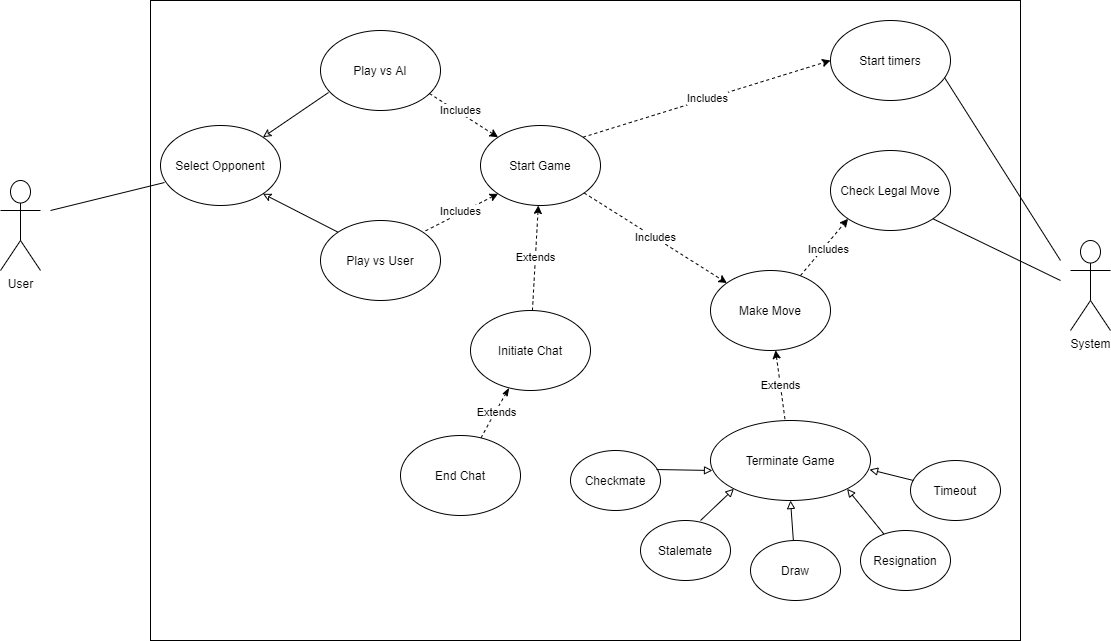
\includegraphics[width=40em,height=30em]{UseCaseDiagram.png}
                \caption{UML Use Case Diagram}
                \label{fig:usecase}
            \end{figure}
            \FloatBarrier

    \subsection{Functional Requirements}
        This section of the SRS contains all of the functional software requirements. The functional requirements detailed here enable designers to design a system that satisfies these requirements, and enable testers to test that the system satisfies these requirements.
        
        \begin{enumerate}[{UC}1.]
        	\item \textbf{\sout{Select Opponent} \textcolor{red}{Join Chat Room}}
        	\begin{enumerate}[{FR}1.]
        	    \item The user shall connect to the web application server.
        		\item \sout{The user shall be immediately presented with the option of playing with an ``AI'' or ``Online Player'' in the middle of their screen. They shall use the labeled buttons to choose between the two options in order to proceed.} \textcolor{red}{The user shall be presented with a welcome screen.}
        		\item \textcolor{red}{The system shall present the user with options to input a username and room name as well as an option to join the specified chat room.}
        		\item \textcolor{red}{If the user attempts to join a chat room before inputting both a username and room name then the system shall prompt them to enter a username and room name. If the user attempts to join a chat room after inputting a username and room name, then the system shall send the user input data to the server and connect the user to the specified chat room. If a chat room with the specified name does not exist, it shall be created.}
        	\end{enumerate}
        	
        	\item \textbf{\sout{Play Against Live Opponent}}
        	\begin{enumerate}[{FR}1., resume]
        		\item \sout{If a user decides to ``Play Against a Live Opponent'' the system shall pair them against a user with the same invite link.}
        		\item \sout{While the system is awaiting another player, the system shall be present the user with the options to ``Quit'', or ``Play Against AI''.}
        		\item \sout{If a user decides to ``Quit'' or ``Play Against AI'' the current game shall be terminated.}
        		\item \sout{If a user selects the ``Quit'' option, the system shall return them to the ``Select Opponent'' use case.}
        		\item \sout{If a user selects the ``Play Against AI'' option, the system shall send them to the ``Play Against AI'' use case.}
        		\item \sout{The system shall present the players with a loading screen while the application is initializing the game. The loading screen shall last no longer than 5 seconds.}
        		\item \sout{Once initialized, the system shall present the players with a view of the board and transfer to the ``Start Game'' use case.}
        		\item \sout{If a user requests to start a game on any server with 15 concurrent games, the system shall reject the request and return to the ``Select Opponent'' use case.}
        	\end{enumerate}
        	
        	\item \textbf{\sout{Play Against AI}}
        	\begin{enumerate}[{FR}1., resume]
        		\item \sout{If a user selects ``Play Against AI'' the system shall immediately transfer to the ``Start Game'' use case.}
                \item \sout{While playing against the AI the system shall have no option to initiate chat.}
        		\item \sout{If a user requests to start a game on any server with 15 concurrent games, the system shall reject the request and return the user to the ``Select Opponent'' use case.}
        	\end{enumerate}
        	
        	\item \textbf{Start Game}
        	\begin{enumerate}[{FR}1., resume]
        		\item \sout{If the user chooses ``AI'' from the ``Select Opponent'' use case, the server shall connect to an AI player and arbitrarily assign black or white to each player.}
        		\item \sout{If the user chooses ``Online Player'' from the ``Select Opponent'' use case, a shareable link shall be created with which a player can join the server. If a player joins, each player shall be arbitrarily assigned black or white.}
        		\item The board and pieces shall be initialized, and the orientation of the board will be determined based on the colour of the users pieces. 
        		\item The timer shall be initialized with a countdown of 10 minutes for each player, and the game control is dependent on the player with the white pieces.
        		\item The system shall give exclusive control to the player with the white pieces and start that player's timer.
        	\end{enumerate}
        	
        	\item \textbf{Make Move}
        	\begin{enumerate}[{FR}1., resume]
        		\item The system shall not allow the player to make a move until their opponent has played a move, with the exception of the first move of the game.
        		\item If a player clicks a piece, holds the mouse down, drags the piece to a square, and releases the mouse, the system shall register an attempted move.
        		\item The application shall confirm that the move is legal as defined by the rules of the game. 
        		\item If the attempted move is legal, the move shall be sent to the server and the opposite player shall be given control.
        		\item If the attempted move is not legal, the move shall not be sent to the server and the player shall retain control.
        		\item The `Terminate Game` use case shall be checked after every move is made.
        		\item If the game is not terminated, the timer for the other player shall resume.
        	\end{enumerate}
        	
        	\item \textbf{Check Legal Move}
        	\begin{enumerate}[{FR}1., resume]
        		\item The application shall register the move the user has made, and check the program logic to determine if the move can be made.
        		\item The move is then reflected in the board state and the opponent may now make their move.
        		\item Only one player will be allowed to make a move at once.
        	\end{enumerate}
        	
        	\item \textbf{Initiate Chat}
        	\begin{enumerate}[{FR}1., resume]
        		\item The system shall present the user with an option to ``Start Chat'' to start a chat.
        		\item If ``Start Chat'' is selected, the system shall open a chat window for both players.
        		\item If both players click on the ``Start Chat'' button simultaneously then the system shall only register one of the selections.
        		\item The ``Start Chat'' button shall be replaced by an ``End Chat'' button.
        	\end{enumerate}
        	
        	\item \textbf{End Chat}
        	\begin{enumerate}[{FR}1., resume]
        		\item The system shall present the user with an option to ``End Chat'' at any time once a chat has started.
        		\item If the chat is ended by one player the chat shall be disabled for both players. The ``End Chat'' button shall be replaced by the ``Start Chat'' button.
        		\item If both players click on the ``End Chat'' button simultaneously then the system shall only register one of the selections.
        		\item If the ``End Chat'' option is selected, the system shall clear all previous chat data.
        	\end{enumerate}
        	
        	\item \textbf{Start Timers}
        	\begin{enumerate}[{FR}1., resume]
        		\item Once a game has been confirmed a timer shall be started by the system.
        		\item The timer shall be set for a total of 10 minutes per player.
        		\item The timer shall begin for a player once it is their turn to move and will pause on their opponents turn.
        	\end{enumerate}
        	
        	%This should be split into a bunch of use cases like we did for select opponent
        	\item \textbf{Terminate Game}
        	\begin{enumerate}[{FR}1., resume]
        	    \item The system will have checks to establish if the game shall be terminated with the appropriate use case possibilities. These include the Checkmate, Stalemate, Draw, Resignation, and Timeout use cases.
        	\end{enumerate}
        	
        	\item \textbf{Checkmate}
        	\begin{enumerate}[{FR}1., resume]
        		\item The system shall determine if the opposing player is in `Check` \cite{ChessRules} (state where the King is under attack) and has no legal moves for the King. This shall result in a victory with `Checkmate` for the current player.
        	\end{enumerate}
        
        	\item \textbf{Stalemate}
        	\begin{enumerate}[{FR}1., resume]
        		\item The system shall determine if the opponent player is not in `Check` and has also no legal moves. This shall result in a draw with `Stalemate` for both players.
        	\end{enumerate}
        	
        	\item \textbf{Draw}
        	\begin{enumerate}[{FR}1., resume]
        		\item The system shall present the user with the `Offer Draw` button to offer a draw to the opponent. The draw must be accepted to end the game.
        	\end{enumerate}
        	
        	\item \textbf{Resignation}
        	\begin{enumerate}[{FR}1., resume]
        	    \item The system shall present the user with a decision to end the game with the `Resign` button. This shall immediately end the game.
        	\end{enumerate}
        	
        	\item \textbf{Timeout}
        	\begin{enumerate}[{FR}1., resume]
        		\item The system shall determine if the user is out of time. This causes that player to lose the game.
        	\end{enumerate}
        \end{enumerate}
    
\section{Non-functional Requirements}

    \subsection{Look and Feel Requirements}
    % Begin SubSection
    
    \subsubsection{Appearance Requirements}
    % Begin SubSubSection
    \begin{enumerate}[{LF}1., leftmargin=2\parindent]
    	\item The system shall use white, \sout{black, and brown} \textcolor{red}{light blue, light green, and dark grey} as its primary colours.
    	\item The system shall use a minimalist design.
    \end{enumerate}
    % End SubSubSection
    
    \subsubsection{Style Requirements}
    \begin{enumerate}[{LF}1., leftmargin=2\parindent, resume]
    	\item The game shall have a calm and intuitive feel as users will be concentrated on making moves under a time constraint, making distractions undesirable.
    	\item \sout{The game shall include sound-effects to inform that a move has been made.}
    	\item The game shall not include background music.
    \end{enumerate}
    % End SubSubSection
    
    % End SubSection
    
    \subsection{Usability and Humanity Requirements}
    % Begin SubSection
    
    \subsubsection{Ease of Use Requirements}
    % Begin SubSubSection
    \begin{enumerate}[{UH}1., leftmargin=2\parindent]
        \item The game shall not require any intricate keyboard presses or fast mouse movements.
        \item The product shall be easy to use by 10 year old children. Ninety percent of a sample test panel of 10 year old children shall be able to successfully play a move within 5 minutes of starting a game.
    \end{enumerate}
    % End SubSubSection
    
    \subsubsection{Personalization and Internationalization Requirements}
    % Begin SubSubSection
    \begin{enumerate}[{UH}1., leftmargin=2\parindent, resume]
    	\item The game shall only display information in English.
    \end{enumerate}
    % End SubSubSection
    
    \subsubsection{Learning Requirements}
    % Begin SubSubSection
    \begin{enumerate}[{UH}1., leftmargin=2\parindent, resume]
    	\item The product shall be able to be used by members of the public over 10 years of age with no previous training.
    	Ninety percent of a sample test panel of the public over 10 years of age shall be able to start a game and move a piece within 5 minutes of accessing the product.
    	\item \sout{Instructions shall be in place to teach the user the rules of the game. Eighty percent of a sample test panel of the public over 12 years of age shall understand how to move each piece within 1 hour of accessing the product.}
    \end{enumerate}
    % End SubSubSection
    
    \subsubsection{Understandability and Politeness Requirements}
    % Begin SubSubSection
    \begin{enumerate}[{UH}1., leftmargin=2\parindent, resume]
    	\item All symbols and words shall be naturally understandable by the user community and shall be similar to historically used Chess symbols \cite{ChessHistory}. 
    \end{enumerate}
    % End SubSubSection
    
    \subsubsection{Accessibility Requirements}
    % Begin SubSubSection
    \begin{enumerate}[{UH}1., leftmargin=2\parindent, resume]
    	\item System shall follow guidelines for correct colour contrast ratio for text to the background as stated in the WCAG \cite{WCAG}.
    \end{enumerate}
    % End SubSubSection
    
    \subsection{Performance Requirements}
    % Begin SubSection
    
    \subsubsection{Speed and Latency Requirements}
    % Begin SubSubSection
    \begin{enumerate}[{PR}1., leftmargin=2\parindent]
    	\item The average time between player input and visual game response shall be less than 0.25 seconds.
    	\item The maximum time between player input and visual game response shall be less than 2 seconds.
    	\item The maximum time between a player input and that player's timer pausing shall be less than 0.1 seconds.
    \end{enumerate}
    % End SubSubSection
    
    \subsubsection{Safety-Critical Requirements}
    % Begin SubSubSection
    \ N/A. The system shall have no safety-critical components or hazards.
    % End SubSubSection
    
    \subsubsection{Precision or Accuracy Requirements}
    % Begin SubSubSection
    \begin{enumerate}[{PR}1., leftmargin=2\parindent, resume]
    	\item All timer values shall be accurate to \sout{one decimal place} \textcolor{red}{the nearest integer}.
    	\item All material score values will be accurate to the nearest integer.
    \end{enumerate}
    % End SubSubSection
    
    \subsubsection{Reliability and Availability Requirements}
    % Begin SubSubSection
    \begin{enumerate}[{PR}1., leftmargin=2\parindent, resume]
    	\item The product shall be available for use 24 hours per day, 360 days per year on average.
    \end{enumerate}
    % End SubSubSection
    
    \subsubsection{Robustness or Fault-Tolerance Requirements}
    % Begin SubSubSection
    \begin{enumerate}[{PR}1., leftmargin=2\parindent, resume]
    	\item The product shall reconnect the player to the \sout{game they were playing} \textcolor{red}{chat room they were connected to} if they lose and regain connection to the server.
    \end{enumerate}
    % End SubSubSection
    
    \subsubsection{Capacity Requirements}
    % Begin SubSubSection
    \begin{enumerate}[{PR}1., leftmargin=2\parindent, resume]
    	\item The product shall require a minimum amount of 2GB of RAM to function effectively.
    \end{enumerate}
    % End SubSubSection
    
    \subsection{Operational and Environmental Requirements}
    % Begin SubSection
    
    \subsubsection{Installability Requirements}
    % Begin SubSubSection
    \ N/A. The system shall require no installation for access and use.
    % End SubSubSection
    
    \subsubsection{Requirements for Interfacing with Adjacent Systems}
    % Begin SubSubSection
    \begin{enumerate}[{OE}1., leftmargin=2\parindent]
        \item The application shall interface with an external server to make requests to the back-end of the application.
    \end{enumerate}
    % End SubSubSection
    
    \subsubsection{Productization Requirements}
    % Begin SubSubSection
    \begin{enumerate}[{OE}1., leftmargin=2\parindent, resume]
    	\item The product shall be deployed to a public website where users shall have access to it.
    \end{enumerate}
    % End SubSubSection
    
    \subsubsection{Release Requirements}
    % Begin SubSubSection
    \begin{enumerate}[{OE}1., leftmargin=2\parindent, resume]
    	\item The product shall be tested for possible bugs and issues, and will accordingly be fixed and redeployed to the product's website on a case-by-case basis. 
    \end{enumerate}
    % End SubSubSection
    
    % End SubSection
    
    \subsection{Maintainability and Support Requirements}
    % Begin SubSection
    
    \subsubsection{Maintenance Requirements}
    % Begin SubSubSection
    \begin{enumerate}[{MS}1., leftmargin=2\parindent]
    	\item The product shall be maintained actively until the end of the semester.
    \end{enumerate}
    % End SubSubSection
    
    \subsubsection{Supportability Requirements}
    % Begin SubSubSection
    \begin{enumerate}[{MS}1., leftmargin=2\parindent, resume]
        \item \sout{The product shall come with an accessible set of instructions on the web-application and in the repository for rules of the game.}
        \item \sout{The product shall provide users with a way of contacting the developers in order to report any bugs or issues they encounter.}
    \end{enumerate}

    \subsubsection{Adaptability Requirements}
    % Begin SubSubSection
    \begin{enumerate}[{MS}1., leftmargin=2\parindent, resume]
    	\item The program shall be accessible from any internet browser on a computer or mobile device.
    	\item The product shall be deployed onto an external platform.
    \end{enumerate}
    % End SubSubSection
    
    % End SubSection
    
    \subsection{Security Requirements}
    % Begin SubSection
    
    \subsubsection{Access Requirements}
    % Begin SubSubSection
    \begin{enumerate}[{SR}1., leftmargin=2\parindent]
    	\item Any user shall be able to access and play the game.
    	\item The product repository shall only be accessible by the developers, TAs, and the professor.
    	\item Only the developers of the project shall be able to modify the files, domain, and the database of the product.
    \end{enumerate}
    % End SubSubSection
    
    \subsubsection{Privacy Requirements}
    % Begin SubSubSection
    \begin{enumerate}[{SR}1., leftmargin=2\parindent, resume]
    	\item There shall be no data collected on users outside of the moves they input.
    \end{enumerate}
    % End SubSubSection
    
    \subsection{Legal Requirements}
    % Begin SubSection
    
    \subsubsection{Standards Requirements}
    % Begin SubSubSection
    \begin{enumerate}[{LR}1., leftmargin=2\parindent]
    	\item The product shall be developed using the Airbnb JavaScript Style Guide \cite{AirbnbStyle}.
    \end{enumerate}

\section{Project Issues}

    \subsection{Open Issues}
        \textcolor{red}{The project uses a new version of React, which does not have full support from all testing dependencies, so testing React components is difficult.}
        
    \subsection{Off-the-Shelf Solutions}
        \textcolor{red}{There are other available products that provide similar and greater functionality to the application. Examples of this are websites like Chess.com and Lichess.}
        
    \subsection{Tasks}
        \textcolor{red}{The tasks for this project are set by the deliverable schedule in the course outline for Software Engineering 3XA3. These tasks include: The problem statement, development plan, requirements document, proof of concept demonstration, test plan, design documents, revision 0 demonstration, final demonstration, and test report.}

    \subsection{Risks}
        \textcolor{red}{There are two main risks that are likely to occur in the development of this project.} The first and biggest risk is that intended features of the product may not be completed within the time-frame for the project. This could cause the design of the system to be worse than if the product was designed without those features in mind. This risk is likely to occur, specifically with the AI and multiplayer features of the product.\\
        
        Another risk is that certain capacities will be measured inaccurately, such as server capacity. This will likely be due to a lack of resources and a lack of knowledge around best practices.\\
        
        \sout{A lack of testing in the project might lead to more errors and unexpected results. It is important to discover as many bugs as possible before the final demonstration, which causes the software to be more reliable and easy to use. There is a risk that there may be uncaught errors and bugs in the program that could negatively affect the user experience.}
        
    \subsection{Costs}
        \textcolor{red}{The main cost for the system is the time of the development team and other stakeholders. However, there are other costs that could be incurred, such as having to purchase licensing for any software libraries used or purchasing a deployment server for the system.}

    \subsection{Waiting Room}
        \textcolor{red}{Multiplayer functionality that allows two users in the same chat room to start a game together or for a player to join a queue of online players.}\\
        
        \textcolor{red}{An option to join a random chat room that has at least one other user already connected.} \\
        
        \textcolor{red}{An option to play against an AI instead of another player.} \\
        
    \subsection{Ideas for Solutions}
        \textcolor{red}{Multiplayer functionality can be added similarly to the chat feature. The system would store individual board states for each player as well as either black or white, and each move would be passed between players. Whenever a move was made the board state would be updated accordingly.} \\
        
        \textcolor{red}{An option to join a populated chat room could be added by storing a list of all chat rooms in use and then returning a random one when called, allowing the user to join that room.}\\
        
        \textcolor{red}{An AI would have to be implemented, and options to play against the AI instead of another player would have to be added to the main screen.}

\newpage    
\bibliographystyle{plainnat}
\bibliography{citations}

\end{document}
